%% LyX 2.0.4 created this file.  For more info, see http://www.lyx.org/.
%% Do not edit unless you really know what you are doing.
\documentclass[oneside,dutch]{amsart}
\usepackage[T1]{fontenc}
\usepackage[latin9]{inputenc}
\usepackage[a4paper]{geometry}
\geometry{verbose,tmargin=3cm,bmargin=3cm,lmargin=2cm,rmargin=2cm}
\setlength{\parskip}{\smallskipamount}
\setlength{\parindent}{0pt}
\usepackage{float}
\usepackage{amsthm}
\usepackage{graphicx}
\graphicspath{{Figures/}}

\makeatletter

%%%%%%%%%%%%%%%%%%%%%%%%%%%%%% LyX specific LaTeX commands.
%% A simple dot to overcome graphicx limitations
\newcommand{\lyxdot}{.}


%%%%%%%%%%%%%%%%%%%%%%%%%%%%%% Textclass specific LaTeX commands.
\numberwithin{equation}{section}
\numberwithin{figure}{section}

\makeatother

\usepackage{babel}
\begin{document}

\title{Michelson en Morley}


\author{N.G. Schultheiss}

\maketitle

\section{Inleiding}

Deze module is direct te volgen vanaf de vierde klas. In deze module
wordt uitgelegd hoe Michelson en Morley er achter kwamen dat er geen
snelheden groter dan de lichtsnelheid mogelijk waren.


\section{Michelson en Morley}

Bij schuine botsingen mogen we in het klassieke geval gebruik maken
van het feit dat snelheden en dus ook impulsen vectorieel op te tellen
zijn. Het is de vraag of dit altijd mag. We beginnen met het volgende
gedachten\-experiment.

Als je een kanaal van precies 2,5{[}km{]} lang neemt en je vaart met
een boot met precies 5{[}km/h{]} op en neer, dan duurt de reis precies
1 uur. Hierna zetten we een sluis open en het water begint met precies
0,5{[}km/h{]} te stromen. Heen vaart de boot tegen de stroom in. Ten
opzichte van de oever wordt de snelheid 4,5{[}km/h{]}, dit is te berekenen
door het verschil in snelheid te nemen. Terug is de snelheid ten opzichte
van de oever 5,5{[}km/h{]}, dit is te berekenen door de snelheden
op te tellen. De heenreis duurt nu 33 minuten en 30 seconden. De terugreis
duurt 26 minuten en 40 seconden. De hele reis duurt door het stromen
van het water dus 10 seconden langer. We kunnen dus kijken of het
medium (in dit geval water) een snelheid heeft, door te meten hoelang
een reis duurt. (Uiteraard wil je weten of ik geen fout heb gemaakt
en reken je het even na.)

In de $19^{e}$ eeuw werd er over het algemeen van uitgegaan dat licht
een golf was die zich in het medium ``aether'' voortbewoog. Naar
analogie van het kanaalverhaal verzonnen Albert Michelson en Edward
Morley het volgende experiment om op verge\-lijk\-bare wijze met
licht te kijken hoe snel wij ons ten opzichte van de ``aether''
voortbewegen. 

\begin{figure}[H]
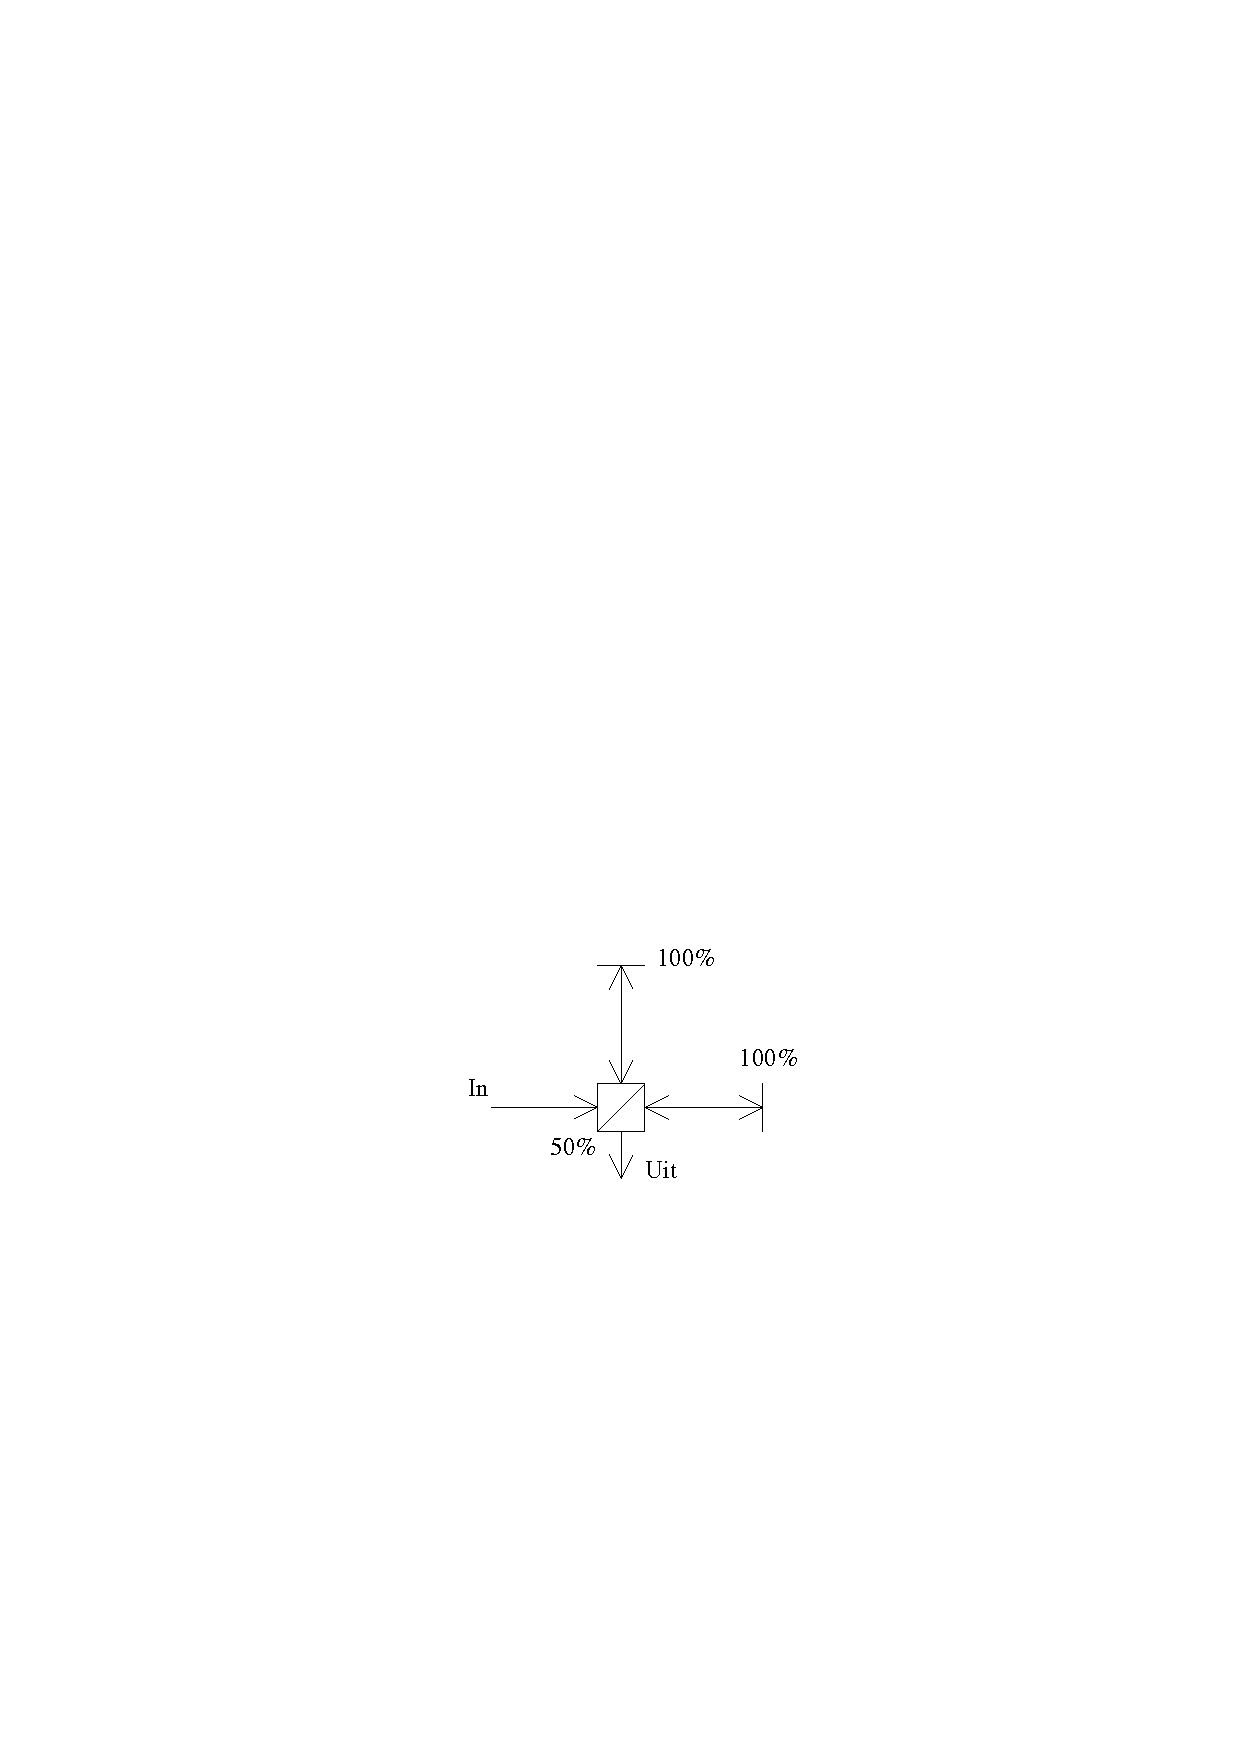
\includegraphics[scale=1]{MM}

\caption{De Michelson en Morley interferometer}
\end{figure}


Een lichtpuls werd door een half doorlatende spiegel gesplitst in
twee pulsen. Deze twee lichtpulsen liepen langs twee verschillende
wegen (bijvoorbeeld Noord/Zuid en Oost/West). Iedere weg heeft dan
een eigen snelheid ten opzichte van de aether. Daarna werden de pulsen
weer samengevoegd en konden Michelson en Morley zien of de lichtpulsen
elkaar uitdoofden (in tegenfase) of niet (in fase). Door de lengte
van een van de wegen een heel klein beetje te veranderen is dit in
te stellen.

Opdracht 1: \emph{Wat voor licht gebruik je het liefst: wit of gekleurd? }

Door in een kaarsvlam een oplossing van keukenzout te spuiten krijg
je monochromatisch licht. Eventueel kun je dit met twee kaarsen en
een keukenzout oplossing experimenteel bepalen. Je kunt kijken of
de ene kaarsvlam een schaduw heeft van de andere kaarsvlam.

Opdracht 2: \emph{Doe dit experiment. Wat mag je concluderen als je
dit vergelijkt met een kaars zonder keukenzoutoplossing? }

Opdracht 3: \emph{Hoe kun je de opstelling het beste instellen? In
fase of in tegenfase?}

Hierna verdraaiden ze de opstelling. In feite gaat dit vanzelf omdat
de aarde als geheel draait. De wegen krijgen nu een andere snelheid
ten opzichte van het medium en dus ook ten opzichte van het licht.
Het was te verwachten dat ze dus iets anders zagen. Dit mede omdat
de uitdoving bij een halve trillingstijd van het licht al ver\-andert.
Helaas veranderde er niets en moesten Michelson en Morley tot de conclusie
komen dat het licht altijd even snel gaat. Blijkbaar kunnen we snelheden
in de buurt van de lichtsnelheid dus niet zomaar optellen.

Opdracht 4: \emph{Bereken hoe snel de aarde aan de evenaar rondraait
en vergelijk dit met de lichtsnelheid.}

Opdracht 5: \emph{De aarde draait ook nog rond de zon. Vergelijk deze
snelheid ook met de lichtsnelheid.}

Opdracht 6: \emph{Schat hoe groot de opstelling van Michelson en Morley
moet zijn. (Hoe\-veel (halve, kwart?) golven licht moet de weg zijn?
Hoeveel meter is dat? Hoe zat het met de echo van geluid?)}

Opdracht 7: \emph{Controleer experimenteel of Michelson en Morley
gelijk hadden.}
\end{document}
